\documentclass{article}
\RequirePackage{amsfonts,amssymb,amsbsy,amsmath}
\usepackage{epsfig,longtable}
\usepackage{listings}
%\usepackage[pdftex]{hyperref}
%\usepackage[pdftex]{graphicx}
\textheight     9.0in \textwidth      6.0in \oddsidemargin  0.0in
\evensidemargin 0.0in \topmargin      -.2in
\parskip        6pt

\DeclareMathOperator{\diag}{diag}

\def\bb{{\beta}}
\def\b{\mbox{\boldmath$\beta$}}
\def\x{\mbox{\boldmath$\xi$}}
\def\no{\noindent}
\def\DD{{\Delta}}
\def \Ac {{\cal A}}



\newtheorem{theo}{Theorem}[section]
\newtheorem{cor}{Corollario}[section]
\newtheorem{lem}{Lemma}[section]
\newtheorem{defn}{Definition}[section]
\newtheorem{ex}{\small \bf Esercizio}[section]
\newtheorem{exa}{\sc \bf Example}[section]
\newtheorem{rem}{\sc Remark}[section]



\def\proof{{\bf Proof.}\quad}
\def \x {{\bf x}}
\def \a {{\bf a}}
\def \b {{\bf b}}
\def \c {{\bf c}}
\def \zero {{\bf 0}}
\def \y {{\bf y}}
\def \b {{\bf b}}
\def \f {{\bf f}}
\def \e {{\bf e}}
\def \w {{\bf w}}
\def \u {{\bf u}}
\def \v {{\bf v}}
\def \t {{\bf t}}
\def \z {{\bf z}}
\def \g {{\bf g}}

\def \xs {{\bar {x}}}
\def \ys {{\bar {y}}}
\def \gs {{\bar {\gamma}}}
\def \ml {{|\lambda|}}
\def \CC {{\mathbb{C}}}
\def \RR {{\mathbb{R}}}
\def \ZZ {{\mathbb{Z}}}
\def \NN {{\mathbb{N}}}
\def \barD {{  \overline  \Delta}}



\def \doty {\dot {\bf {y} }}
\def \ddoty {\ddot {\bf {y} }}
\def \dotv {\dot {\bf {v} }}
\def \eps {\varepsilon}
\def \lt {\tilde{\lambda}}
\newcommand{\balpha}{\mbox{\boldmath $\alpha$}}
\newcommand{\bbeta}{\mbox{\boldmath $\beta$}}
\newcommand{\bdelta}{\mbox{\boldmath $\delta$}}
\newcommand{\brho}{\mbox{\boldmath $\rho$}}
\newcommand{\btau}{\mbox{\boldmath $\tau$}}
\newcommand{\bxi}{\mbox{\boldmath $\xi$}}
\newcommand{\cbxi}{\mbox{\boldmath $\hat \xi$}}

\def \no {\noindent}



\def \pmatrix{ \left( \begin{array} }
\def \endpmatrix{ \end{array} \right) }
\hyphenation{me-thod} \hyphenation{me-thods} \hyphenation{exact}
\hyphenation{ar-bi-tra-ri-ly} \hyphenation{dia-go-nal-ly}
\begin{document}

 \vspace*{1cm}


\begin{center}
{\Huge BVPTWP Manual}\\[5mm]
{\Large J. R. CASH$^{\ast}$, D. HOLLEVOET$^{\star}$, F. MAZZIA$^{\dag}$,  A. M. NAGY$^{\ddagger}$}\\
[5mm]
{\Large $^{\ast}$\small Department of Mathematics,
Imperial College, South Kensington, London SW7, England.}\\ e-mail: \texttt{j.cash@imperial.ac.uk}\\[5mm]
{\Large $^{\star}$\small Vakgroep Toegepaste Wiskunde en Informatica, Universiteit Gent, Krijgslaan 281 S9, 9000 Gent.}\\
e-mail:
\texttt{davy.hollevoet@ugent.be}\\[5mm]
{\Large $^{\dag}$\small Dipartimento di Matematica, Universit\`a di Bari, Via Orabona 4, 70125 Bari (Italy).}\\
e-mail:
\texttt{mazzia@dm.uniba.it}\\[5mm]
{\Large $^{\ddagger}$\small Dipartimento di Matematica, Universit\`a di Bari, Via Orabona 4, 70125 Bari (Italy)\\ Department of Mathematics, Benha University, 13518 Benha (Egypt). } \\
e-mail: \texttt{abdelhameed\_nagy@yahoo.com}\\
\end{center}



\newpage
\section*{Contents}
\begin{tabular*}{\textwidth}{@{}lcrcr@{}}
\multicolumn{5}{@{}c@{}}{\rule{\textwidth}{0mm}}\\
\phantom{I}1.\; Introduction                       &&&& {\sl \pageref{intro}} \\[2mm]
\phantom{I}2.\; BVPTWP Package     &&&& {\sl \pageref{bvptwp}} \\[2mm]
\phantom{II}2.1.\; Installation                       &&&& {\sl \pageref{Insta}} \\[2mm]
\phantom{II}2.2.\; How to solve test set problems using a MATLAB solver     &&&& {\sl \pageref{solver}} \\[2mm]
\phantom{II}2.3.\; Examples     &&&& {\sl \pageref{Exa}} \\[2mm]
%\multicolumn{5}{c}{\pmb{\em Test problems collected so far:}}\\[3mm]
\end{tabular*}


\section{Introduction}\label{intro}
In recent years much attention has been given to the numerical solution of boundary
value problems in ODEs. Of particular interest has been the solution of  singularly perturbed
problems. This type of problem arises in various fields of science and engineering such as fluid
mechanics, physics, chemistry, mechanics, chemical reactor theory, convection diffusion processes, 
optimal control and other branches of applied mathematics. Singular perturbation problems depend on 
the presence of a small, positive parameter which provides a multi-scale character to the solution. That is
there are layer(s) where the solution varies very rapidly in some parts of the region of integration and varies
slowly in some other parts. \texttt{bvptwp} is a MATLAB program that calculates an approximate solution for
two-point Boundary Value Problems that may or may not be singularly perturbed.
The general BVP is of the form:
\begin{equation}\label{bvp1}
y'=f(x,y),  \quad    a \leq  x \leq b
\end{equation}
\begin{equation}\label{bvp2}
g(y(a),y(b)) = 0,
\end{equation}
where $ g = ( g_{1}, g_{2},\cdot\cdot\cdot,g_{n})^{T}$ is a vector functions.
The functions $f$ and $g_{i}$ are assumed to be differentiable.
The problem must be posed as a first-order system. This requirement is not unduly restrictive,
however, since standard techniques can be used to convert an $n$th-order equation to a system
of $n$ first-order equations. For example, the second-order   singularly
perturbed  problem
\begin{equation}
 \lambda y''=f(x,y,y'),\quad 0 < x < 1, \quad y(0) = \alpha, \quad y(1) = \beta,
\end{equation}
where $0 <\lambda \ll 1,\, x \in \mathbb{R},\,$
can be converted to the following first-order system:
\begin{equation*}
\begin{array}{l}
u' = z, \\
z' = \dfrac{1}{\lambda}f(x,u,z), \\
 u(0) = \alpha, \quad u(1) = \beta.\\
\end{array}
\end{equation*}


\section{BVPTWP Package}\label{bvptwp}
The purpose of this section is to give a brief introduction to the use of the routines
in Matlab by means of some fairly simple examples. In particular, we show how to
compute an approximate solution and how to evaluate these solutions by various graphical
tools. Although the examples given below do not touch upon all the features of
\texttt{bvptwp} tools, they illustrate the fundamental ideas underlying the
package.
\subsection{Installation}\label{Insta}

Extract the contents of the archive \texttt{bvptwp\_1.0.zip} into a directory of your choice, e.g.
\texttt{bvptwp-path}. This newly created directory should now be added to the MATLAB path. This
can be done temporarly (for one MATLAB session) by executing
\begin{verbatim}
>> addpath ('bvptwp-path/bvptwp_1.0')
\end{verbatim}
on the MATLAB command line (be sure to use single quotes). The package can also be added to the MATLAB path permanently via
\texttt{File/Set Path...} and \texttt{Add Folder...}. The \texttt{bvptwp} package is now ready for use.

\subsection{How to solve a problem using bvptwp}\label{solver}
The solver \texttt{bvptwp} is an interface for solving BVPs by using
a deferred correction scheme based on LOBATTO methods (\texttt{twpbvp\_l}),
a deferred correction scheme based on MIRK methods
(\texttt{twpbvp\_m}) or a continuation strategy based on
LOBATTO methods (\texttt{acdc}). The interface is built such that it can
 be used in a MATLAB environment like the well-known solvers \texttt{bvp4c} and \texttt{bvp5c}.
 The three codes can also be used with a hybrid mesh selection strategy based on
 conditioning by means of the corresponding variants \texttt{twpbvpc\_l}, \texttt{twpbvpc\_m} and \texttt{acdcc}.

To solve a problem with $m$ components, \texttt{\texttt{bvptwp.m}} can be
invoked with three parameters: 

\begin{verbatim}
>> SOL = bvptwp(odefun, bcfun, solinit)
\end{verbatim}

or four parameters:

\begin{verbatim}
>> SOL = bvptwp(odefun, bcfun, solinit, options)
\end{verbatim}

\begin{itemize}
 \item \texttt{odefun}: function handle \\
  The provided function implements $f(x,y)$ of the differential equation. If option \texttt{Vectorized}
  is not enabled, this function is given a scalar $x$ and a vector $y$ and should return a
  $m \times 1$ matrix.
 \item \texttt{bcfun}: function handle \\
  The provided function computes $bc(y(a),y(b))$ at the boundaries.
 \item \texttt{solinit}: struct\\
 A compatible structure for \texttt{solinit} can be constructed with the function
\texttt{bvpinit} from MATLAB. Afterwards, an additional field  \texttt{fixpnt} can be added to the
 structure obtained, which specifies additional mesh points in which the solution should
be calculated.
%  This structure provides an initial guess of the solution. Can be constructed with \texttt{bvpinit}.
 % Additionally, fixed points can be specified through this structure.
\item \textit{(Optional)} \texttt{options}: struct \\
  A structure that specifies options for the solver. Can be constructed with \texttt{bvptwpset}.
  \end{itemize}


The output \texttt{SOL} is a structure with
\begin{itemize}
         \item \texttt{SOL.x}:  last mesh selected by   \texttt{bvptwp}.
         \item  \texttt{SOL.y}: approximation to $y(x)$ at the mesh points of
         \texttt{SOL.x}.
         \item \texttt{SOL.solver}: \texttt{'twpbvp\_m'} or \texttt{'twpbvp\_l'}
         or \texttt{'acdc'} or \texttt{'twpbvpc\_m'} or \texttt{'twpbvpc\_l'} or
         \texttt{'acdcc'}.
         \item \texttt{SOL.lambda}: the final value of the continuation 
                            parameter used (only for \texttt{acdc},
                            \texttt{acdcc)}.
         \item  \texttt{SOL.iflbvp}:  
         \begin{itemize} 
                     \item[$0$]: the code solved the problem.
                   
                     \item[$-1$]: the code solved a problem with a different
                            continuation parameter  (only for \texttt{acdc},
                            \texttt{acdcc}).
 
                    \item[$1$]: tha code failed (maximum number of meshpoints
                          reached).
                          
                     \item[$2$]: the code failed (maximum number of possible
                           meshes reached, default 100, only for
                           \texttt{twpbvpc\_m}, \texttt{twpbvpc\_l}).
                           
                     \item[$3$]: the code failed (maximum number of continuation
                          steps reached, only for  \texttt{acdc},
                          \texttt{acdcc}). 
                     \item[$4$]: the code failed (unknown error).
                     \end{itemize}
                          
         \item \texttt{SOL.condpar}: information about the conditioning
         parameters (only for \texttt{twpbvpc\_m}, \texttt{twpbvpc\_l},
         \texttt{acdcc})
                        \begin{itemize}
                         \item \texttt{SOL.condpar.kappa}: conditioning of the
                         bvp in inf norm.
                         
                           \item \texttt{SOL.condpar.kappa1}: conditioning
                         related to changes in the initial values (inf norm).

                           \item \texttt{SOL.condpar.kappa2}: conditioning
                         related to the Green's function (inf norm).

                           \item \texttt{SOL.condpar.gamma1}: conditioning
                         related to changes in the initial values (1 norm).

                           \item \texttt{SOL.condpar.sigma}: stiffness
                           parameter.

                           \item \texttt{SOL.condpar.stabcond}: 1 or 0 if the
                         conditioning parameters stabilized.
                         \end{itemize}
         \item \texttt{SOL.stats}:  Computational cost, statistics and
         information about the maximum scaled error computed.

\end{itemize}


\begin{verbatim}
>> SOL = bvptwp(odefun, bcfun, solinit, options)
\end{verbatim}

 solves as above with default parameters
 replaced by values in \texttt{options}, a structure created with the
 \texttt{bvptwpset} function. To reduce the run time greatly, use
 \texttt{options} to supply a function for evaluating the Jacobian and/or
 Jvectorize.
 
\subsubsection{Options that can be specified in parameter \texttt{options}
(defaults are marked with \{\}).}

Options shared with \texttt{bvpc4.m} and \texttt{bvpc5.m}:

\begin{itemize}
 \item \texttt{Vectorized}: \texttt{on|\{off\}} \\
  Set to \texttt{'on'} when \texttt{odefun} can be evaluated at several points at once.
  When enabled, the function handle is invoked as \texttt{odefun}
  $([x_1, \ldots, x_n],[y_1, \ldots, y_n])$ and is expected to return an $m
  \times n$ matrix.
 \item \texttt{FJacobian}: function handle \texttt{df}\\
  If provided, \texttt{df} implements the Jacobian $\partial f/\partial y$ of the problem.
  The function provided will be invoked as \texttt{df(x,y)} with scalar x and vector y.
  In the absence of this option, the Jacobian is calculated numerically with
  \texttt{odenumjac} from MATLAB.
 \item \texttt{BCJacobian}: function handle \texttt{dbc}\\
  A function handle that computes the partial derivatives $\partial bc/\partial y_a$
  and $\partial bc/\partial y_b$ of the boundary conditions.
  Calls to this function will be made as \texttt{dbc(ya,yb)} and two $m \times
  m$ matrices are expected as output.
  \item \texttt{NMax}: positive integer \{$\lfloor 50000/m \rfloor$\} \\
  Maximum number of mesh points allowed.
  \item \texttt{RelTol}: positive scalar \{$1e$-3\} or vector. Relative tolerance for the error. If \texttt{RelTol} is a vector a different tolerance is
used for all components of the solution. The value 0 means that the corresponding
component is not used in the error estimation.
  \item \texttt{Stats}: \texttt{on|\{off\}} \\
  Show a few statistics at the end of the computations.


  Additional options provided by \texttt{bvptwp.m}:
 \item \texttt{Solver}:\texttt{'twpbvp\_m'|\{'twpbvp\_l'\}
 (for linear problems) |'acdc'|\{'twpbvpc\_m'\} (for
 non linear problems) |'twpbvpc\_l'  |'acdcc'} \\
  Use deferred correction based on MIRK
 (\texttt{twpbvp\_m}) or LOBATTO methods (\texttt{twpbvp\_l}) or a continuation
 strategy based on LOBATTO methods (\texttt{acdc}) or their implementation
 based on conditioning (\texttt{twpbvpc\_m,twpbvpc\_m,acdcc}).  
 \item \texttt{LambdaStart}: positive scalar \{0.5\}\\  Starting value for the continuation parameter, used only for \texttt{acdc(c)} solver.
 \item \texttt{LambdaMin}: positive scalar \{$1e$-5\}\\  Final value for the continuation parameter, used only for \texttt{acdc(c)} solver.
 \item \texttt{JVectorized}: \texttt{on|\{off\}} \\
  Set to \texttt{'on'} if the function handle \texttt{df} specified for \texttt{FJacobian}
   is capable of computing the Jacobian at several points at once. If enabled, this setting
    will cause \texttt{df} to be called as \texttt{df}$([x_1, \ldots, x_n],[y_1,
    \ldots, y_n])$. This function should return a $m \times m \times n$ matrix.
 \item \texttt{Linear}: \texttt{on|\{off\}} \\
  Used to indicate whether or not the problem is linear. If enabled, the problem is solved taking
  into account the linear behavior.
 \item \texttt{MaxNumberOfMeshes}: positive integer \{100\}\\
  This is the maximum number of different meshes that could be used during
  computation. It is important to avoid loops.
  \item \texttt{MaxNumberOfContStep}: positive integer \{150\} \\
  This is the maximum number of continuation steps  (only for
  \texttt{acdc/acdcc} solvers).
 \item \texttt{Debug}: \texttt{on|\{off\}} \\
  Enable or disable debugging information (very verbose!).
\end{itemize}

 
\pagebreak

\subsection{Examples}
\label{Exa}
\subsubsection{Example 1}
We consider the following singularly perturbed, linear two-point boundary
value problem
\begin{equation}\label{ex6}
\begin{array}{l} \epsilon y'' + x y' = -\epsilon \pi^2 \cos(\pi x) - \pi x \sin(\pi x), \\
y(-1) = -2,\quad y(1)=0\end{array}
\end{equation}
whose exact solution is
$y(x)=\cos(\pi x) +\mbox{erf}(x/\sqrt{2\epsilon})/\mbox{erf}(1/\sqrt{2
\epsilon})$.

The following MATLAB function illustrates how \texttt{bvptwp.m} can be
used to solve example~\eqref{ex6}.

\begin{figure}[t]
\centerline{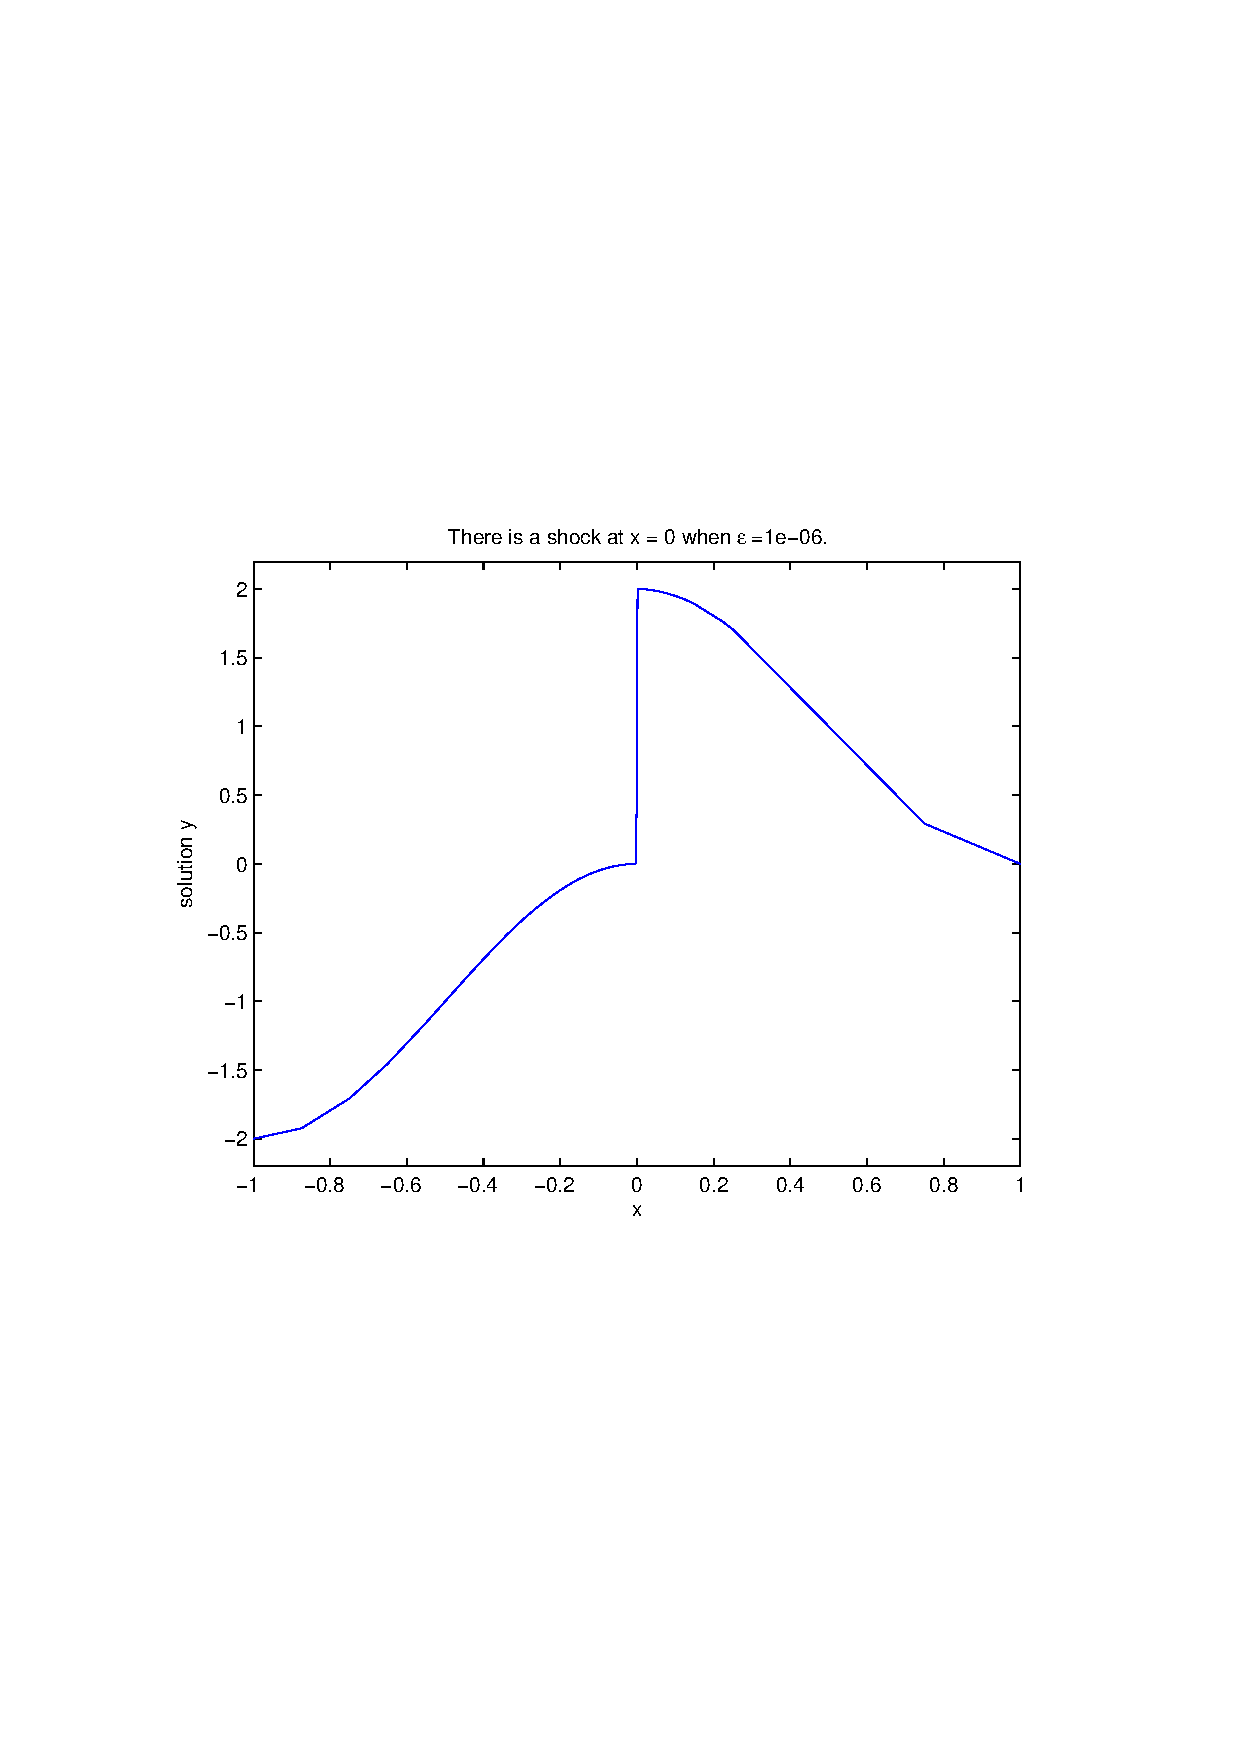
\includegraphics[height=6cm]{shock_bvptwp}}
\caption{Output of the example shock\_bvptwp.}
\end{figure}

\lstset{language=MATLAB}
\lstset{commentstyle=\textit,basicstyle=\small}

\begin{lstlisting}[fontadjust]{}
function shock_bvptwp(solver)
%shock_bvptwp  The solution has a shock layer near x = 0
%   This is an example used in U. Ascher, R. Mattheij, and R. Russell,
%   Numerical Solution of Boundary Value Problems for Ordinary Differential
%   Equations, SIAM, Philadelphia, PA, 1995,  to illustrate the mesh
%   selection strategy of COLSYS. 
%
%   For 0 < e << 1, the solution of 
%
%       e*y'' + x*y' = -e*pi^2*cos(pi*x) - pi*x*sin(pi*x)
%
%   on the interval [-1,1] with boundary conditions y(-1) = -2 and y(1) = 0
%   has a rapid transition layer at x = 0.
%
%   For this problem,
%   analytical partial derivatives are easy to derive and the solver benefits
%   from using them.  
%
%   By default, this example uses the 'twpbvpc_l' solver. Use syntax 
%   SHOCK_BVPTWP(solver) to solve this problem with the another solver
%     available solvers are: 'twpbvp_m', 'twpbvpc_m', 'twpbvp_l', 'twpbvpc_l',
%                            'acdc', 'acdcc'
%
%   See also bvptwp, bvptwpset, bvptwpget, bvpinit, function_handle.
%   THIS MFILE IS ADAPDET FORM THE SHOCKBVP OF
%   Jacek Kierzenka and Lawrence F. Shampine
%   Copyright 1984-2007 The MathWorks, Inc.
%   $Revision: 1.10.4.3 $  $Date: 2007/05/23 18:53:57 $

  if nargin < 1
    solver = 'twpbvpc_l';
  end


  % The differential equations written as a first order system and the
  % boundary conditions are coded in shockODE and shockBC, respectively. Their
  % partial derivatives are coded in shockJac and shockBCJac and passed to the
  % solver via the options. The option 'Vectorized' instructs the solver that
  % the differential equation function has been vectorized, i.e.
  % shockODE([x1 x2 ...],[y1 y2 ...]) returns [shockODE(x1,y1) shockODE(x2,y2) ...].
  % Such coding improves the solver performance.

  options = bvptwpset(	'FJacobian',@shockJac,'BCJacobian',@shockBCJac,...
			'Solver',solver,'RelTol',[1e-4;0],'Linear','on');

  % A guess for the initial mesh and the solution
  %sol = bvpinit([-1 -0.5 0 0.5 1],[1 0]);
  solinit =bvpinit(linspace(-1,1,9),zeros(1,2));

  e = 1e-6;
  if  strcmp(solver,'acdc')|| strcmp(solver,'acdcc')
      options=bvptwpset(options,'Lambdamin',e);
  end

  sol = bvptwp(@shockODE,@shockBC,solinit,options);

  % The final solution
  figure;
  plot(sol.x,sol.y(1,:));
  axis([-1 1 -2.2 2.2]);
  title(['There is a shock at x = 0 when \epsilon =' sprintf('%.e',e) '.']);
  xlabel('x');
  ylabel('solution y');

  % -----------------------------------------------------------------------
  % Nested functions -- e is shared with the outer function.
  %

  function dydx = shockODE(x,y,ExtraArgs)
    %SHOCKODE  Evaluate the ODE function (vectorized)
    if nargin==3
      e=ExtraArgs;
    end

    pix = pi*x;
    dydx = [  y(2,:)
	      (-x.*y(2,:) - e*pi^2*cos(pix) - pix.*sin(pix))/e ];
  end
  % -----------------------------------------------------------------------

  function res = shockBC(ya,yb,ExtraArgs)
    %SHOCKBC  Evaluate the residual in the boundary conditions
    if nargin==3
      e=ExtraArgs;
    end

    res = [ ya(1)+2
            yb(1)  ];
  end
  % -----------------------------------------------------------------------

  function jac = shockJac(x,y,ExtraArgs)
    %SHOCKJAC  Evaluate the Jacobian of the ODE function
    %  x and y are required arguments.
    if nargin==3
      e=ExtraArgs;
    end
    jac = [ 0   1
            0 -x/e ];
  end
  % -----------------------------------------------------------------------

  function [dBCdya,dBCdyb] = shockBCJac(ya,yb,ExtraArgs)
    %SHOCKBCJAC  Evaluate the partial derivatives of the boundary conditions
    %  ya and yb are required arguments.
    if nargin==3
      e=ExtraArgs;
    end

    dBCdya = [ 1 0
               0 0 ];

    dBCdyb = [ 0 0
               1 0 ];
  end
end  % shock_bvptwp

\end{lstlisting}



\pagebreak

\subsubsection{Example 2}

A second example compares the final mesh obtained from four solvers without continuation. The problem under
consideration is
\begin{equation}
\label{ex2}
\begin{array}{l}
  y'' = \epsilon sinh(\epsilon y), \\
  y(0) = 0,\quad y(1)=1.
\end{array}
\end{equation}
The following MATLAB function illustrates how \texttt{bvptwp.m} can be
used to solve  example~\eqref{ex2}.
\begin{lstlisting}[fontadjust]{}
function sinh_bvptwp()
% sinh_bvptwp
%  compares the final mesh obtained from four solvers without continuation.
% The problem under  consideration is
%    y'' = e sinh(e y),
%   with boundary conditions
%    y(0) = 0,    y(1)=1.
%
% For this problem: 
%      Function f is vectorized
%      Analytical Jacobians are not implemented
%      RelTol is the same for both components
%      Printing statistics after solving is enabled
%
    options = bvptwpset('Vectorized','on',...
		'RelTol',1e-8,...
		'Linear','off',...
		'NMax',1000,...
		'Stats','on');

    % A guess for the initial mesh and the solution
    sol = bvpinit(linspace(0,1,18),[0,0]);

    e = 5.32675;

    % uses deferred correction with MIRK methods
    options = bvptwpset(options,'Solver','twpbvp_m');
    sol1 = bvptwp(@sinhODE,@sinhBC,sol,options);

    % uses deferred correction with MIRK methods and conditioning
    options = bvptwpset(options,'Solver','twpbvpc_m');
    sol2 = bvptwp(@sinhODE,@sinhBC,sol,options);

    % uses deferred correction with Lobatto methods
    options = bvptwpset(options,'Solver','twpbvp_l');
    sol3 = bvptwp(@sinhODE,@sinhBC,sol,options);

    % uses deferred correction with Lobatto methods and conditioning
    options = bvptwpset(options,'Solver','twpbvpc_l');
    sol4 = bvptwp(@sinhODE,@sinhBC,sol,options);



    %%% Nested functions, e is shared with the outer function

    function dydx = sinhODE(x,y)
        % Evaluate the ODE function (vectorized)
        dydx = [ y(2,:)
                 e*sinh(e*y(1,:)) ];
    end

    function res = sinhBC(ya,yb)
        % Evaluate the residual in the boundary conditions
        res = [ ya(1)
                yb(1)-1 ];
    end
end

\end{lstlisting}

The output is:

\begin{lstlisting}[fontadjust]{}
-------------------------------------
Solver twpbvp_m.
The solution was obtained on a mesh of 42 points.
The maximum scaled error  is  6.897e+00. 
There were 60 calls to the ODE function. 
There were 23 calls to the BC function. 
-------------------------------------
Solver twpbvpc_m.
The solution was obtained on a mesh of 47 points.
The maximum scaled error  is  5.208e-01. 
There were 60 calls to the ODE function. 
There were 23 calls to the BC function. 
-------------------------------------
Solver twpbvp_l.
The solution was obtained on a mesh of 40 points.
The maximum scaled error  is  5.307e+00. 
There were 60 calls to the ODE function. 
There were 22 calls to the BC function. 
-------------------------------------
Solver twpbvpc_l.
The solution was obtained on a mesh of 41 points.
The maximum scaled error  is  3.515e+00. 
There were 60 calls to the ODE function. 
There were 22 calls to the BC function. 
\end{lstlisting}

\end{document} 